\section{Softwarearchitektur und Design}


\subsection{Grundlagen der Softwarearchitektur}

\begin{concept}{Grundlagen und Überblick}
\begin{itemize}
    \item \textbf{Business Analyse:}
    \begin{itemize}
        \item Domänenmodell und Kontextdiagramm
        \item Requirements (funktional und nicht-funktional)
        \item Vision und Stakeholder
    \end{itemize}
    
    \item \textbf{Architektur:}
    \begin{itemize}
        \item Logische Struktur des Systems
        \item Technische Konzeption
        \item Qualitätsanforderungen
    \end{itemize}
    
    \item \textbf{Entwicklung:}
    \begin{itemize}
        \item Use Case / User Story Realisierung
        \item Design-Klassendiagramm (DCD)
        \item Implementierung und Tests
    \end{itemize}
\end{itemize}

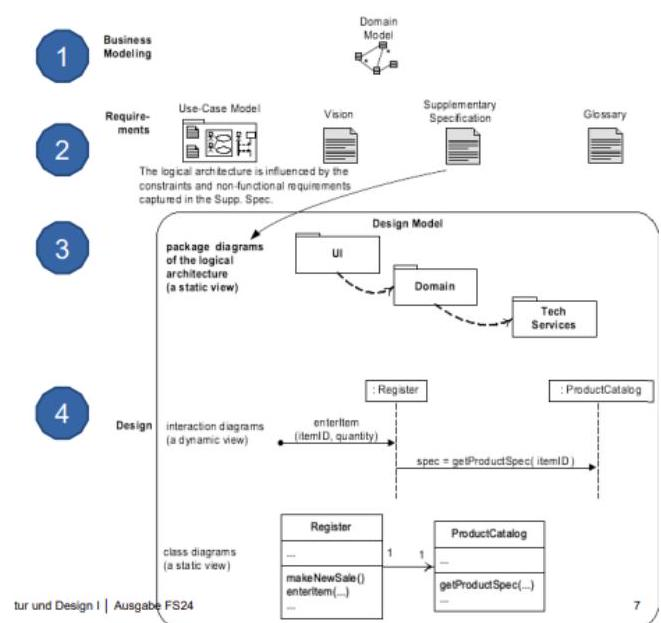
\includegraphics[width=\linewidth]{images/2024_12_29_0d1d7b5551ea1b4b41bdg-07(2)}
\end{concept}

\begin{definition}{Softwarearchitektur}\\
Die Architektur eines Softwaresystems definiert:

\begin{itemize}
    \item \textbf{Grundlegende Entscheidungen:}
    \begin{itemize}
        \item Programmiersprachen und Plattformen
        \item Aufteilung in Teilsysteme und Komponenten
        \item Schnittstellen zwischen Komponenten
    \end{itemize}
    
    \item \textbf{Strukturelle Aspekte:}
    \begin{itemize}
        \item Verantwortlichkeiten der Teilsysteme
        \item Abhängigkeiten zwischen Komponenten
        \item Einsatz von Basis-Technologien/Frameworks
    \end{itemize}
    
    \item \textbf{Qualitätsaspekte:}
    \begin{itemize}
        \item Erfüllung nicht-funktionaler Anforderungen
        \item Maßnahmen für Performance, Skalierbarkeit etc.
        \item Fehlertoleranz und Ausfallsicherheit
    \end{itemize}
\end{itemize}
\end{definition}

\begin{concept}{Architekturanalyse}\\
erfolgt iterativ mit den Anforderungen (Twin Peaks Model):

\begin{itemize}
    \item \textbf{Anforderungsanalyse:}
    \begin{itemize}
        \item Analyse funktionaler und nicht-funktionaler Anforderungen
        \item Prüfung der Qualität und Stabilität der Anforderungen
        \item Identifikation von Lücken und impliziten Anforderungen
    \end{itemize}
    
    \item \textbf{Architekturentscheidungen:}
    \begin{itemize}
        \item Abstimmung mit Stakeholdern
        \item Berücksichtigung von Randbedingungen
        \item Vorausschauende Planung für zukünftige Änderungen
    \end{itemize}
\end{itemize}

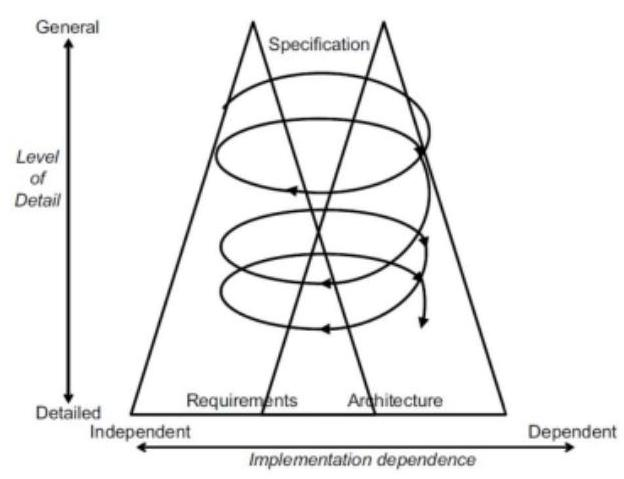
\includegraphics[width=0.9\linewidth]{images/2024_12_29_0d1d7b5551ea1b4b41bdg-08}
\end{concept}

\begin{theorem}{Qualitätsanforderungen}\\
\textbf{ISO 25010:}
\begin{itemize}
    \item Hierarchische Struktur für nicht-funktionale Anforderungen
    \item Definierte Hauptcharakteristiken und Subcharakteristiken
    \item Messbare Metriken für jede Anforderung
    \item Ermöglicht präzise Formulierung und Verifikation
\end{itemize}

\textbf{FURPS+:}
\begin{itemize}
    \item \textbf{F}unctionality (Funktionalität)
    \item \textbf{U}sability (Benutzerfreundlichkeit)
    \item \textbf{R}eliability (Zuverlässigkeit)
    \item \textbf{P}erformance (Leistung)
    \item \textbf{S}upportability (Wartbarkeit)
    \item \textbf{+}: Implementation, Interface, Operations, Packaging, Legal
\end{itemize}
\end{theorem}

\subsection{Architekturdesign}

\begin{concept}{Modulkonzept}\\
Ein Modul (Baustein, Komponente) wird bewertet nach:
\begin{itemize}
    \item \textbf{Kohäsion:} Innerer Zusammenhang
    \item \textbf{Kopplung:} Externe Abhängigkeiten
\end{itemize}

\textbf{Eigenschaften:}
\begin{itemize}
    \item Autarkes Teilsystem
    \item Minimale externe Schnittstellen
    \item Enthält alle benötigten Funktionen/Daten
    \item Verschiedene Formen: Paket, Library, Service
\end{itemize}
\end{concept}

\begin{definition}{Schnittstellen}\\
Module kommunizieren über definierte Schnittstellen:

\begin{itemize}
    \item \textbf{Exportierte Schnittstellen:}
    \begin{itemize}
        \item Definieren angebotene Funktionalität
        \item Vertraglich garantierte Leistungen
        \item Einzige nach außen sichtbare Information
    \end{itemize}
    
    \item \textbf{Importierte Schnittstellen:}
    \begin{itemize}
        \item Von anderen Modulen benötigte Funktionalität
        \item Definieren Abhängigkeiten
        \item Basis für Kopplung
        \item Sollten minimiert werden (Low Coupling)
    \end{itemize}
\end{itemize}
\end{definition}

\begin{concept}{Architektursichten (4+1 View Model)}\\
Verschiedene Perspektiven auf die Architektur:

\begin{itemize}
    \item \textbf{Logical View:} End-User, Functionality
    \begin{itemize}
        \item Funktionalität des Systems
        \item Schichten, Subsysteme, Pakete
        \item Klassen und Schnittstellen
    \end{itemize}
    
    \item \textbf{Process View:} Integrators, Performance, Scalability
    \begin{itemize}
        \item Laufzeitverhalten
        \item Prozesse und Threads
        \item Performance und Skalierung
    \end{itemize}

    \item \textbf{Development View:} Programmers, Software Management
    \begin{itemize}
        \item Implementierungsstruktur
        \item Quellcode-Organisation
        \item Build und Deployment
    \end{itemize}
    
    \item \textbf{Physical View:} System Engineers, Topology, Communications
    \begin{itemize}
        \item Hardware-Topologie
        \item Verteilung der Software
        \item Netzwerkkommunikation
    \end{itemize}
\end{itemize}
    
\textbf{+1: Scenarios:}
    \begin{itemize}
        \item Wichtige Use Cases
        \item Validierung der Architektur
        \item Integration der anderen Views
    \end{itemize}

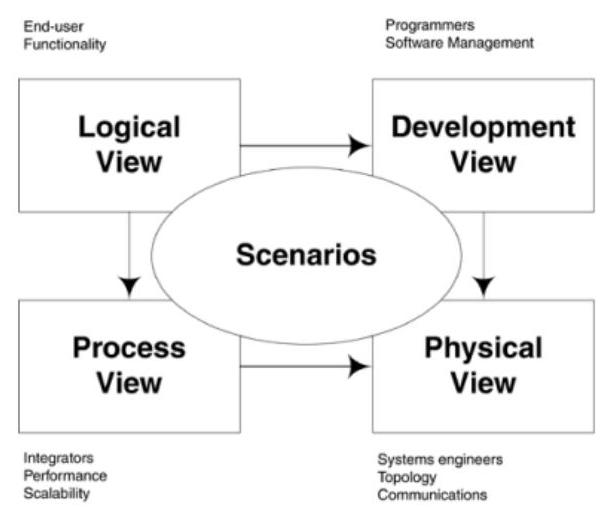
\includegraphics[width=0.9\linewidth]{images/2024_12_29_0d1d7b5551ea1b4b41bdg-09}
\end{concept}

\begin{concept}{Architekturprinzipien}
Grundlegende Prinzipien für gute Architektur:

\textbf{Separation of Concerns:}
\begin{itemize}
    \item Trennung von Verantwortlichkeiten
    \item Klare Modulgrenzen
    \item Reduzierte Komplexität
\end{itemize}

\textbf{Information Hiding:}
\begin{itemize}
    \item Kapselung von Implementierungsdetails
    \item Definierte Schnittstellen
    \item Änderbarkeit ohne Seiteneffekte
\end{itemize}

\textbf{Loose Coupling:}
\begin{itemize}
    \item Minimale Abhängigkeiten
    \item Austauschbarkeit
    \item Unabhängige Entwicklung
\end{itemize}
\end{concept}


\begin{corollary}{Qualitätskriterien und deren Umsetzung}\\
Strategien zur Erfüllung von Qualitätsanforderungen:

\textbf{Performance:}
\begin{itemize}
    \item Effiziente Ressourcennutzung (Resource Pooling, Caching)
    \item Optimierte Verarbeitung (Parallelisierung, Lazy Loading)
\end{itemize}

\textbf{Skalierbarkeit:}
\begin{itemize}
    \item Dynamische Anpassung (horizontale/vertikale Skalierung)
    \item Effiziente Lastverteilung (Load Balancing, Partitionierung)
\end{itemize}

\textbf{Wartbarkeit:}
\begin{itemize}
    \item Klare Strukturen (Separation of Concerns, Modularisierung)
    \item Verbesserte Codequalität (Information Hiding, Standardisierung)
\end{itemize}

\textbf{Zuverlässigkeit:}
\begin{itemize}
    \item Fehlerresistenz (Redundanz, Fehlertoleranz)
    \item Prävention und Wiederherstellung (Monitoring, Backup/Recovery)
\end{itemize}

\textbf{Verfügbarkeit:}
\begin{itemize}
    \item Ausfallschutz (Redundanz, Failover-Mechanismen)
    \item Überwachung/Stabilisierung (Health Monitoring, Circuit Breaker)
\end{itemize}

\textbf{Modularität:}
\begin{itemize}
    \item Gut definierte Grenzen (klare Modulgrenzen, hohe Kohäsion)
    \item Minimale Abhängigkeiten zwischen Modulen
\end{itemize}

\textbf{Testbarkeit:}
\begin{itemize}
    \item Einfachheit von Tests (Isolation, Mockbarkeit)
    \item Automatisierung und Skalierung von Tests
\end{itemize}

\textbf{Änderbarkeit:}
\begin{itemize}
    \item Anpassungsfähigkeit (Lokalisierung, Erweiterbarkeit)
    \item Sicherstellung der Kompatibilität (Backward Compatibility)
\end{itemize}

\textbf{Erweiterbarkeit:}
\begin{itemize}
    \item Flexible Architekturen (offene Schnittstellen, Plugin-Systeme)
    \item Serviceorientierung für modulare Erweiterungen
\end{itemize}
\end{corollary}

\subsection{Architekturprozess und Best Practices}
%todo: make easier to understand, remove redundant information, make more concise, add examples from Wissenssicherungen and missing information from the slides

\begin{formula}{Best Practices im Architekturentwurf}\\
\textbf{1. Analyse und Planung}
\begin{itemize}
    \item Anforderungen priorisieren
    \item Qualitätsziele definieren
    \item Constraints identifizieren
    \item Stakeholder einbinden
\end{itemize}

\textbf{2. Design-Prinzipien}
\begin{itemize}
    \item Separation of Concerns
    \item Single Responsibility
    \item Information Hiding
    \item Don't Repeat Yourself (DRY)
\end{itemize}

\textbf{3. Strukturierung}
\begin{itemize}
    \item Klare Schichtenarchitektur
    \item Definierte Schnittstellen
    \item Lose Kopplung
    \item Hohe Kohäsion
\end{itemize}

\textbf{4. Dokumentation}
\begin{itemize}
    \item Architekturentscheidungen
    \item Begründungen
    \item Alternativen
    \item Trade-offs
\end{itemize}
\end{formula}

\subsubsection{Gesamter Architekturprozess}

\begin{definition}{Architekturprozess-Komponenten}\\
\textbf{Architekturanalyse:}
\begin{itemize}
    \item Erster Schritt im Architekturprozess
    \item Analyse der funktionalen und nicht-funktionalen Anforderungen
    \item Identifikation von Qualitätszielen
    \item Parallel zur Anforderungserhebung (Twin Peaks)
\end{itemize}

\textbf{Architektur-Entscheidungen:}
\begin{itemize}
    \item Konkrete Beschlüsse basierend auf der Analyse
    \item Technologiewahl und Strukturierung
    \item Dokumentation und Begründung
    \item Einschließlich verworfener Alternativen
\end{itemize}

\textbf{Architektur-Entwurf:}
\begin{itemize}
    \item Praktischer Gestaltungsprozess
    \item Anwendung von Architekturmustern
    \item Umsetzung von Qualitätsanforderungen
    \item Erstellung konkreter Artefakte
\end{itemize}

\textbf{Architektur-Review:}
\begin{itemize}
    \item Systematische Überprüfung
    \item Meist durch externe Experten
    \item Prüfung der Anforderungserfüllung
    \item Identifikation von Schwachstellen
\end{itemize}

\textbf{Architektur-Evaluation:}
\begin{itemize}
    \item Bewertung anhand definierter Kriterien
    \item Quantitative und qualitative Analyse
    \item Szenario-basierte Prüfung
    \item Bewertung von Qualitätsattributen
\end{itemize}
\end{definition}

\begin{KR}{Gesamter Architekturprozess}\\
\textbf{1. Initiale Phase}
\begin{itemize}
    \item Architekturanalyse durchführen
    \item Grundlegende Entscheidungen treffen
    \item Ersten Entwurf erstellen
\end{itemize}

\textbf{2. Iterative Verfeinerung}
\begin{itemize}
    \item Review durchführen
    \item Evaluation vornehmen
    \item Anpassungen basierend auf Feedback
\end{itemize}

\textbf{3. Kontinuierliche Verbesserung}
\begin{itemize}
    \item Regelmäßige Reviews
    \item Neue Anforderungen einarbeiten
    \item Technische Schulden adressieren
\end{itemize}

\textbf{4. Dokumentation}
\begin{itemize}
    \item Entscheidungen festhalten
    \item Architektur dokumentieren
    \item Änderungen nachverfolgen
\end{itemize}

\textbf{5. Qualitätssicherung}
\begin{itemize}
    \item Architektur-Konformität prüfen
    \item Performance-Tests durchführen
    \item Sicherheitsaudits durchführen
\end{itemize}
\end{KR}

\begin{example2}{Gesamter Architekturprozess}\\
    %todo: add example
\end{example2}


\begin{KR}{Architekturanalyse}\\
\textbf{1. Anforderungen sammeln}
\begin{itemize}
    \item Funktionale Anforderungen gruppieren
    \item Nicht-funktionale Anforderungen identifizieren
    \item Randbedingungen dokumentieren
\end{itemize}

\textbf{2. Qualitätsziele definieren}
\begin{itemize}
    \item Messbare Kriterien festlegen
    \item Priorisierung vornehmen
    \item Trade-offs identifizieren
\end{itemize}

\textbf{3. Einflussfaktoren analysieren}
\begin{itemize}
    \item Technische Faktoren
    \item Organisatorische Faktoren
    \item Wirtschaftliche Faktoren
\end{itemize}
\end{KR}

\begin{example2}{Architekturanalyse}\\
    %todo: add example    
\end{example2}

\begin{KR}{Architektur-Entscheidungen}\\
\textbf{1. Alternativen identifizieren}
\begin{itemize}
    \item Mögliche Lösungen sammeln
    \item Vor- und Nachteile analysieren
    \item Machbarkeit prüfen
\end{itemize}

\textbf{2. Bewertungskriterien}
\begin{itemize}
    \item Erfüllung der Anforderungen
    \item Technische Umsetzbarkeit
    \item Kosten und Aufwand
\end{itemize}

\textbf{3. Entscheidung dokumentieren}
\begin{itemize}
    \item Begründung
    \item Konsequenzen
    \item Verworfene Alternativen
\end{itemize}
\end{KR}

\begin{corollary}{Architektur-Entscheidungen dokumentieren}\\
\textbf{1. Entscheidung festhalten}
\begin{itemize}
    \item Dokumentation der getroffenen Architekturentscheidungen
    \item Begründungen und Alternativen
    \item Auswirkungen und Konsequenzen
\end{itemize}

\textbf{2. Strukturierte Dokumentation}
\begin{itemize}
    \item Einheitliches Format für alle Entscheidungen
    \item Verwendung von Templates
    \item Nachvollziehbare Historie der Entscheidungen
\end{itemize}

\textbf{3. Kommunikation}
\begin{itemize}
    \item Regelmäßige Updates an Stakeholder
    \item Transparenz über getroffene Entscheidungen
    \item Einbindung des gesamten Teams
\end{itemize}

\textbf{4. Review und Anpassung}
\begin{itemize}
    \item Regelmäßige Überprüfung der Entscheidungen
    \item Anpassung bei geänderten Rahmenbedingungen
    \item Lessons Learned dokumentieren
\end{itemize}
\end{corollary}

\begin{example2}{Architektur-Entscheidungen}\\
    %todo: add example    
\end{example2}


\begin{KR}{Architekturentwurf}\\
\textbf{Schritte:}
\begin{enumerate}
    \item Anforderungen analysieren
    \item Architekturstil wählen
    \item Module identifizieren
    \item Schnittstellen definieren
    \item Mit Stakeholdern abstimmen
\end{enumerate}
\end{KR}

\begin{example2}{Architekturentwurf}\\
    %todo: add example
\end{example2}

\begin{KR}{Architektur-Review durchführen}\\
\textbf{Vorgehen:}
\begin{enumerate}
    \item \textbf{Vorbereitung}
    \begin{itemize}
        \item Architektur-Dokumentation zusammenstellen
        \item Review-Team zusammenstellen
        \item Checklisten vorbereiten
    \end{itemize}
    
    \item \textbf{Durchführung}
    \begin{itemize}
        \item Architektur vorstellen
        \item Anforderungen prüfen
        \item Entscheidungen hinterfragen
        \item Risiken identifizieren
    \end{itemize}
    
    \item \textbf{Nachbereitung}
    \begin{itemize}
        \item Findings dokumentieren
        \item Maßnahmen definieren
        \item Follow-up planen
    \end{itemize}
\end{enumerate}

\textbf{Prüfkriterien:}
\begin{itemize}
    \item Anforderungserfüllung
    \item Technische Machbarkeit
    \item Zukunftssicherheit
    \item Best Practices
\end{itemize}
\end{KR}

\begin{example2}{Architektur-Review}\\
    %todo: add example    
\end{example2}



\begin{KR}{Architektur-Evaluation}\\
Systematische Bewertung einer Softwarearchitektur:

\textbf{1. Qualitätsattribute identifizieren}
\begin{itemize}
    \item Performance
    \item Skalierbarkeit
    \item Wartbarkeit
    \item Sicherheit
\end{itemize}

\textbf{2. Szenarien entwickeln}
\begin{itemize}
    \item Normale Nutzung
    \item Grenzfälle
    \item Fehlerfälle
    \item Wartungsszenarien
\end{itemize}

\textbf{3. Architektur analysieren}
\begin{itemize}
    \item Strukturanalyse
    \item Verhaltensanalyse
    \item Trade-off Analyse
\end{itemize}

\textbf{4. Risiken identifizieren}
\begin{itemize}
    \item Technische Risiken
    \item Geschäftsrisiken
    \item Architekturrisiken
\end{itemize}
\end{KR}

\begin{example2}{Architektur-Evaluation}\\
    %todo: add example    
\end{example2}

\subsubsection{Beispiele Architekturentwurf}

\begin{example2}{Typische Prüfungsaufgabe: Architekturanalyse und Entscheidungen}\\
\textbf{Aufgabenstellung:}
Analysieren Sie folgende Anforderungen und leiten Sie architektonische Konsequenzen ab:
\begin{itemize}
    \item System muss 24/7 verfügbar sein
    \item 10.000 gleichzeitige Benutzer
    \item Reaktionszeit unter 1 Sekunde
    \item Jährliche Wartungsfenster maximal 4 Stunden
\end{itemize}

\textbf{Lösung:}
\begin{itemize}
    \item \textbf{Architekturentscheidungen:}
    \begin{itemize}
        \item Verteilte Architektur für Hochverfügbarkeit
        \item Load Balancing für gleichzeitige Benutzer
        \item Caching-Strategien für Performanz
        \item Blue-Green Deployment für Wartung
    \end{itemize}
    
    \item \textbf{Begründungen:}
    \begin{itemize}
        \item Verteilung minimiert Single Points of Failure
        \item Load Balancer verteilt Last gleichmäßig
        \item Caching reduziert Datenbankzugriffe
        \item Blue-Green erlaubt Updates ohne Downtime
    \end{itemize}
\end{itemize}
\end{example2}

\begin{example2}{Architekturentwurf}\\
\textbf{Aufgabe:} Entwerfen Sie die grundlegende Architektur für ein Online-Banking-System.

\textbf{Lösung:}
\begin{itemize}
    \item \textbf{Anforderungsanalyse:}
    \begin{itemize}
        \item Sicherheit (ISO 25010)
        \item Performance (FURPS+)
        \item Skalierbarkeit
    \end{itemize}
    
    \item \textbf{Architekturentscheidungen:}
    \begin{itemize}
        \item Mehrschichtige Architektur
        \item Microservices für Skalierbarkeit
        \item Sicherheitsschicht
    \end{itemize}
    
    \item \textbf{Module:}
    \begin{itemize}
        \item Authentifizierung
        \item Transaktionen
        \item Kontoführung
    \end{itemize}
\end{itemize}
\end{example2}

\begin{example2}{Architektur-Evaluation: Performance}\\
\textbf{Szenario:} Online-Shop während Black Friday

\textbf{Analyse:}
\begin{itemize}
    \item \textbf{Last-Annahmen:}
    \begin{itemize}
        \item 10.000 gleichzeitige Nutzer
        \item 1.000 Bestellungen pro Minute
        \item 100.000 Produktaufrufe pro Minute
    \end{itemize}
    
    \item \textbf{Architektur-Maßnahmen:}
    \begin{itemize}
        \item Caching-Strategie für Produkte
        \item Load Balancing für Anfragen
        \item Asynchrone Bestellverarbeitung
        \item Datenbank-Replikation
    \end{itemize}
    
    \item \textbf{Monitoring:}
    \begin{itemize}
        \item Response-Zeiten
        \item Server-Auslastung
        \item Cache-Hit-Rate
        \item Fehlerraten
    \end{itemize}
\end{itemize}

\begin{lstlisting}[language=Java, style=basesmol]
// Performance-optimierte Produktabfrage
@Cacheable(value = "products")
public ProductDTO getProduct(String id) {
    ProductDTO product = cache.get(id);
    if (product == null) {
        product = repository.findById(id)
                          .map(this::toDTO)
                          .orElseThrow();
        cache.put(id, product);
    }
    return product;
}
\end{lstlisting}
\end{example2}


\pagebreak

\subsection{Architekturmuster und Clean Code}

\begin{concept}{Architekturmuster}\\
Grundlegende Architekturmuster für Software-Systeme:

\begin{itemize}
    \item \textbf{Layered Pattern:} 
    \begin{itemize}
        \item Strukturierung in horizontale Schichten
        \item Klare Trennung der Verantwortlichkeiten
        \item Abhängigkeiten nur nach unten
    \end{itemize}
    
    \item \textbf{Client-Server Pattern:}
    \begin{itemize}
        \item Verteilung von Diensten
        \item Zentralisierte Ressourcen
        \item Mehrere Clients pro Server
    \end{itemize}
    
    \item \textbf{Master-Slave Pattern:}
    \begin{itemize}
        \item Verteilung von Aufgaben
        \item Zentrale Koordination
        \item Parallelverarbeitung
    \end{itemize}
    
    \item \textbf{Pipe-Filter Pattern:}
    \begin{itemize}
        \item Datenstromverarbeitung
        \item Verkettung von Operationen
        \item Wiederverwendbare Filter
    \end{itemize}
    
    \item \textbf{Broker Pattern:}
    \begin{itemize}
        \item Vermittlung zwischen Komponenten
        \item Entkopplung von Diensten
        \item Zentrale Koordination
    \end{itemize}
    
    \item \textbf{Event-Bus Pattern:}
    \begin{itemize}
        \item Asynchrone Kommunikation
        \item Publisher-Subscriber Modell
        \item Lose Kopplung
    \end{itemize}
\end{itemize}
\end{concept}

\begin{KR}{Event-Bus Pattern}
\textbf{Implementierung eines Event-Bus Systems:}

\textbf{1. Event-Bus}

\begin{itemize}
    \item Publisher-Subscriber Mechanismus implementieren
    \item Event-Routing einrichten
    \item Event-Persistenz berücksichtigen
    \item Ordering und Filtering ermöglichen
\end{itemize}

\textbf{2. Publisher}

\begin{itemize}
    \item Event-Typen definieren
    \item Event-Publikation implementieren
    \item Transaktionshandling berücksichtigen
    \item Fehlerbehandlung vorsehen
\end{itemize}

\textbf{3. Subscriber}

\begin{itemize}
    \item Event-Handler implementieren
    \item Idempotenz sicherstellen
    \item Fehlertoleranz einbauen
    \item Dead-Letter-Queue vorsehen
\end{itemize}
\end{KR}

\begin{example2}{Event-Bus Implementation}
\begin{lstlisting}[language=Java, style=basesmol]
// Event Bus
public class EventBus {
    private Map<Class<?>, List<EventSubscriber>> subscribers = new HashMap<>();
    
    public void publish(Event event) {
        List<EventSubscriber> eventSubscribers = subscribers
            .getOrDefault(event.getClass(), Collections.emptyList());
            
        for (EventSubscriber subscriber : eventSubscribers) {
            try {
                subscriber.onEvent(event);
            } catch (Exception e) {
                handleSubscriberError(subscriber, event, e);
            }
        }
    }
    public void subscribe(Class<?> eventType, EventSubscriber subscriber) {
        subscribers.computeIfAbsent(eventType, k -> new ArrayList<>())
                  .add(subscriber);
    }
}
// Publisher
public class OrderService {
    private EventBus eventBus;
    
    public void createOrder(OrderRequest request) {
        Order order = orderRepository.save(
            new Order(request));
            
        eventBus.publish(new OrderCreatedEvent(
            order.getId(),
            order.getCustomerId(),
            order.getTotalAmount(),
            LocalDateTime.now()
        ));
    }
}
// Subscriber
@Component
public class NotificationService implements EventSubscriber {
    private ProcessedEventRepository processedEvents;
    
    @Override
    public void onEvent(Event event) {
        if (!(event instanceof OrderCreatedEvent)) return;
        
        String eventId = event.getId();
        if (processedEvents.exists(eventId)) return;
        
        try {
            sendNotification((OrderCreatedEvent) event);
            processedEvents.save(eventId);
        } catch (Exception e) {
            sendToDeadLetterQueue(event, e);
        }
    }
}
\end{lstlisting}
\end{example2}



\begin{KR}{Layered Pattern}\\
\textbf{Anwendung des Schichtenmusters:}

\textbf{1. Schichten identifizieren}
\begin{itemize}
    \item Präsentationsschicht (UI)
    \item Anwendungsschicht (Application Logic)
    \item Geschäftslogikschicht (Domain Logic)
    \item Datenzugriffsschicht (Data Access)
\end{itemize}

\textbf{2. Regeln definieren}
\begin{itemize}
    \item Kommunikation nur mit angrenzenden Schichten
    \item Abhängigkeiten nur nach unten
    \item Jede Schicht kapselt ihre Implementierung
\end{itemize}

\textbf{3. Schnittstellen festlegen}
\begin{itemize}
    \item Klare Service-Interfaces pro Schicht
    \item Dependency Injection für lose Kopplung
    \item Daten-DTOs für Schichtübergänge
\end{itemize}
\end{KR}

\begin{example2}{Layered Pattern Implementation}
\begin{lstlisting}[language=Java, style=basesmol]
// Presentation Layer
public class CustomerController {
    private CustomerService service;
    
    public CustomerDTO getCustomer(String id) {
        Customer customer = service.findById(id);
        return CustomerDTO.from(customer);
    }
}

// Application Layer
public class CustomerService {
    private CustomerRepository repository;
    
    public Customer findById(String id) {
        validateId(id);
        return repository.findById(id)
        .orElseThrow(CustomerNotFoundException::new);
    }
}

// Domain Layer
public class Customer {
    private CustomerId id;
    private String name;
    private Address address;
    
    public void updateAddress(Address newAddress) {
        validateAddress(newAddress);
        this.address = newAddress;
    }
}

// Persistence Layer
public class CustomerRepository {
    private JpaRepository<Customer, CustomerId> jpaRepo;
    
    public Optional<Customer> findById(String id) {
        return jpaRepo.findById(new CustomerId(id));
    }
}
\end{lstlisting}
\end{example2}

\begin{KR}{Client-Server Pattern}\\
\textbf{Implementierung einer Client-Server Architektur:}

\textbf{1. Server-Design}
\begin{itemize}
    \item Services definieren
    \item Schnittstellen dokumentieren
    \item Sicherheitsaspekte berücksichtigen
    \item Skalierbarkeit einplanen
\end{itemize}

\textbf{2. Client-Design}
\begin{itemize}
    \item Client-Typen festlegen (Thin/Rich/Web)
    \item Fehlerbehandlung implementieren
    \item Offline-Fähigkeit berücksichtigen
    \item Caching-Strategie entwickeln
\end{itemize}

\textbf{3. Kommunikation}
\begin{itemize}
    \item Protokoll wählen (REST, GraphQL, etc.)
    \item API-Versionierung einplanen
    \item Rate Limiting implementieren
    \item Monitoring einrichten
\end{itemize}
\end{KR}

\begin{example2}{Client-Server Implementation}
\begin{lstlisting}[language=Java, style=basesmol]
// Server-Side
@RestController
@RequestMapping("/api/v1")
public class ProductController {
    private final ProductService service;
    
    @GetMapping("/products/{id}")
    public ProductDTO getProduct(@PathVariable String id) {
        return service.findById(id)
            .map(ProductDTO::from)
            .orElseThrow(ProductNotFoundException::new);
    }
}

// Client-Side
public class ProductClient {
    private final WebClient webClient;
    
    public Mono<Product> getProduct(String id) {
        return webClient.get()
                       .uri("/products/{id}", id)
                       .retrieve()
                       .bodyToMono(ProductDTO.class)
                       .map(ProductDTO::toDomain)
                       .onErrorMap(this::handleError);
    }
}
\end{lstlisting}
\end{example2}

\begin{KR}{Master-Slave Pattern}\\
\textbf{Implementierung einer Master-Slave Architektur:}

\textbf{1. Master-Komponente}
\begin{itemize}
    \item Aufgabenverteilung implementieren
    \item Slave-Management einrichten
    \item Fehlertoleranz berücksichtigen
    \item Load Balancing implementieren
\end{itemize}

\textbf{2. Slave-Komponenten}
\begin{itemize}
    \item Aufgabenbearbeitung implementieren
    \item Statusmeldungen einrichten
    \item Fehlerbehandlung implementieren
    \item Recovery-Mechanismen vorsehen
\end{itemize}

\textbf{3. Koordination}
\begin{itemize}
    \item Kommunikationsprotokoll definieren
    \item Synchronisation implementieren
    \item Monitoring einrichten
    \item Failover-Strategien entwickeln
\end{itemize}
\end{KR}

\begin{example2}{Master-Slave Implementation}
\begin{lstlisting}[language=Java, style=basesmol]
// Master
public class TaskMaster {
    private List<SlaveWorker> workers;
    private Queue<Task> taskQueue;
    
    public void distributeTask(Task task) {
        SlaveWorker worker = selectAvailableWorker();
        worker.assignTask(task);
        monitorProgress(worker);
    }
    
    private void handleWorkerFailure(SlaveWorker worker) {
        Task failedTask = worker.getCurrentTask();
        reassignTask(failedTask, getNextAvailableWorker());
    }
}

// Slave
public class SlaveWorker {
    private TaskProcessor processor;
    private WorkerStatus status;
    
    public void assignTask(Task task) {
        status = WorkerStatus.BUSY;
        try {
            Result result = processor.process(task);
            reportSuccess(result);
        } catch (Exception e) {
            reportFailure(e);
        }
        status = WorkerStatus.IDLE;
    }
}
\end{lstlisting}
\end{example2}

\begin{KR}{Pipe-Filter Pattern}
\textbf{Implementierung einer Pipe-Filter Architektur:}

\textbf{1. Filter-Design}
\begin{itemize}
    \item Atomare Transformationen definieren
    \item Ein- und Ausgabeformat festlegen
    \item Fehlerbehandlung implementieren
    \item Unabhängige Verarbeitung sicherstellen
\end{itemize}

\textbf{2. Pipe-Design}
\begin{itemize}
    \item Datentransfer implementieren
    \item Pufferung einrichten
    \item Threading-Modell festlegen
    \item Backpressure berücksichtigen
\end{itemize}

\textbf{3. Pipeline-Konfiguration}
\begin{itemize}
    \item Filter-Reihenfolge definieren
    \item Verzweigungen ermöglichen
    \item Monitoring einrichten
    \item Fehlerszenarien behandeln
\end{itemize}
\end{KR}

\begin{example2}{Pipe-Filter Implementation}
\begin{lstlisting}[language=Java, style=basesmol]
// Filter Interface
public interface Filter<I, O> {
    O process(I input);
}

// Concrete Filter
public class ValidationFilter implements Filter<Data, Data> {
    @Override
    public Data process(Data input) {
        if (!isValid(input)) {
            throw new ValidationException("Invalid data");
        }
        return input;
    }
}

// Pipe Implementation
public class Pipeline<I, O> {
    private List<Filter> filters = new ArrayList<>();
    
    public void addFilter(Filter filter) {
        filters.add(filter);
    }
    
    public O process(I input) {
        Object current = input;
        for (Filter filter : filters) {
            current = filter.process(current);
        }
        return (O) current;
    }
}

// Usage
Pipeline<RawData, ProcessedData> pipeline = new Pipeline<>();
pipeline.addFilter(new ValidationFilter());
pipeline.addFilter(new TransformationFilter());
pipeline.addFilter(new EnrichmentFilter());
ProcessedData result = pipeline.process(rawData);
\end{lstlisting}
\end{example2}

\begin{KR}{Broker Pattern}
\textbf{Implementierung eines Broker Systems:}
\vspace{1mm}\\
\textbf{1. Broker-Komponente}

\begin{minipage}[t]{0.5\textwidth}
\begin{itemize}
    \item Service-Registry implementieren
    \item Request-Routing einrichten
\end{itemize}
\end{minipage}
\begin{minipage}[t]{0.5\textwidth}
\begin{itemize}
    \item Load Balancing implementieren
    \item Service-Discovery ermöglichen
\end{itemize}
\end{minipage}
\vspace{1mm}\\
\textbf{2. Service-Provider}

\begin{minipage}[t]{0.5\textwidth}
\begin{itemize}
    \item Service-Interface definieren
    \item Bei Broker registrieren
\end{itemize}
\end{minipage}
\begin{minipage}[t]{0.5\textwidth}
\begin{itemize}
    \item Health Checks implementieren
    \item Fehlerbehandlung vorsehen
\end{itemize}
\end{minipage}
\vspace{1mm}\\
\textbf{3. Service-Consumer}

\begin{minipage}[t]{0.5\textwidth}
\begin{itemize}
    \item Service-Lookup implementieren
    \item Fehlertoleranz einbauen
\end{itemize}
\end{minipage}
\begin{minipage}[t]{0.5\textwidth}
\begin{itemize}
    \item Caching-Strategie entwickeln
    \item Retry-Mechanismen vorsehen
\end{itemize}
\end{minipage}
\end{KR}

\begin{example2}{Broker Implementation}
\begin{lstlisting}[language=Java, style=basesmol]
public class ServiceBroker {    // Broker
    private Map<String, List<ServiceProvider>> services = new HashMap<>();
    
    public void register(ServiceProvider provider) {
        String serviceType = provider.getServiceType();
        services.computeIfAbsent(serviceType, k -> new ArrayList<>())
                .add(provider);
    }
    public ServiceProvider getProvider(String serviceType) {
        List<ServiceProvider> providers = services.get(serviceType);
        if (providers == null || providers.isEmpty()) {
            throw new ServiceNotFoundException(serviceType);
        }
        return selectProvider(providers); // Load balancing
    }
}
public class ServiceProvider {  // Service Provider
    private String serviceType;
    private String endpoint;
    private HealthCheck healthCheck;
    public Response handleRequest(Request request) {
        try {
            validateRequest(request);
            return processRequest(request);
        } catch (Exception e) {
            return handleError(e);
        }
    }
}
public class ServiceConsumer {  // Service Consumer
    private ServiceBroker broker;
    private Cache cache;
    public Response callService(String serviceType, Request request) {
        Response cached = cache.get(request);
        if (cached != null) return cached;
        return RetryTemplate.execute(() -> {
            ServiceProvider provider = broker.getProvider(serviceType);
            Response response = provider.handleRequest(request);
            cache.put(request, response);
            return response;
        });
    }
}
\end{lstlisting}
\end{example2}


\subsubsection{Clean Architecture}

\begin{concept}{Clean Architecture}\\
Architektur-Prinzipien nach Robert C. Martin:

\textbf{Hauptprinzipien:}
\begin{itemize}
    \item Unabhängigkeit von Frameworks
    \item Unabhängigkeit von UI
    \item Unabhängigkeit von Datenbank
    \item Testbarkeit ohne externe Systeme
\end{itemize}

\textbf{Schichten (von innen nach außen):}
\begin{itemize}
    \item \textbf{Entities:} 
    \begin{itemize}
        \item Zentrale Geschäftsregeln
        \item Unternehmensweit gültig
        \item Höchste Stabilität
    \end{itemize}
    
    \item \textbf{Use Cases:}
    \begin{itemize}
        \item Anwendungsspezifische Geschäftsregeln
        \item Orchestrierung der Entities
        \item Anwendungslogik
    \end{itemize}
    
    \item \textbf{Interface Adapters:}
    \begin{itemize}
        \item Konvertierung von Daten
        \item Präsentation und Controller
        \item Gateway-Implementierungen
    \end{itemize}
    
    \item \textbf{Frameworks \& Drivers:}
    \begin{itemize}
        \item UI-Framework
        \item Datenbank
        \item Externe Schnittstellen
    \end{itemize}
\end{itemize}
\end{concept}

\begin{KR}{Clean Architecture}\\
\textbf{Implementierung der Clean Architecture:}

\textbf{1. Schichten definieren}
\begin{itemize}
    \item \textbf{Entities:}
    \begin{itemize}
        \item Zentrale Geschäftsobjekte identifizieren
        \item Geschäftsregeln definieren
        \item Unabhängig von externen Frameworks
    \end{itemize}
    
    \item \textbf{Use Cases:}
    \begin{itemize}
        \item Anwendungsfälle implementieren
        \item Geschäftslogik orchestrieren
        \item Input/Output Boundaries definieren
    \end{itemize}
    
    \item \textbf{Interface Adapters:}
    \begin{itemize}
        \item Controller implementieren
        \item Presenter erstellen
        \item Gateways definieren
    \end{itemize}
    
    \item \textbf{Frameworks \& Drivers:}
    \begin{itemize}
        \item UI-Framework einbinden
        \item Datenbankzugriff implementieren
        \item Externe Services anbinden
    \end{itemize}
\end{itemize}

\textbf{2. Dependency Rule beachten}
\begin{itemize}
    \item Abhängigkeiten nur nach innen
    \item Interfaces für Richtungsumkehr
    \item DTOs für Datentransfer
\end{itemize}

\textbf{3. Clean Architecture Testing}
\begin{itemize}
    \item Unit Tests für Entities
    \item Use Case Tests ohne externe Systeme
    \item Integrationstests für Adapter
    \item End-to-End Tests für das Gesamtsystem
\end{itemize}
\end{KR}

\columnbreak

\begin{example2}[breakable]{Clean Architecture Implementation}
\begin{lstlisting}[language=Java, style=basesmol]
// Entity Layer
public class Order {
    private OrderId id;
    private CustomerId customerId;
    private Money totalAmount;
    private OrderStatus status;
    
    public void confirm() {
        validateStateForConfirmation();
        this.status = OrderStatus.CONFIRMED;
    }
    
    private void validateStateForConfirmation() {
        if (status != OrderStatus.PENDING) {
            throw new InvalidOrderStateException();
        }
    }
}

// Use Case Layer
public class CreateOrderUseCase implements CreateOrder {
    private final OrderRepository orderRepository;
    private final PaymentGateway paymentGateway;
    
    @Override
    public CreateOrderResponse execute(CreateOrderRequest request) {
        // Business logic
        Order order = new Order(
            request.getCustomerId(),
            request.getAmount()
        );
        
        // Business rules validation
        validateOrder(order);
        
        // Store order
        orderRepository.save(order);
        
        // Process payment
        PaymentResult payment = paymentGateway.process(
            order.getId(),
            order.getTotalAmount()
        );
        
        // Return response
        return new CreateOrderResponse(
            order.getId(),
            payment.getTransactionId()
        );
    }
}

// Interface Adapters Layer
@RestController
public class OrderController {
    private final CreateOrder createOrderUseCase;
    
    @PostMapping("/orders")
    public ResponseEntity<OrderResponse> createOrder(
            @RequestBody OrderRequest request) {
        // Convert request to use case input
        CreateOrderRequest useCaseRequest = 
            mapToUseCaseRequest(request);
        
        // Execute use case
        CreateOrderResponse response = 
            createOrderUseCase.execute(useCaseRequest);
        
        // Convert and return response
        return ResponseEntity.ok(
            mapToApiResponse(response));
    }
}

// Frameworks & Drivers Layer
@Repository
public class JpaOrderRepository implements OrderRepository {
    private final JpaOrderEntityRepository jpaRepo;
    
    @Override
    public void save(Order order) {
        OrderEntity entity = mapToEntity(order);
        jpaRepo.save(entity);
    }
    
    @Override
    public Optional<Order> findById(OrderId id) {
        return jpaRepo.findById(id.getValue())
                     .map(this::mapToDomain);
    }
}
\end{lstlisting}
\end{example2}

\begin{concept}{Clean Architecture Best Practices}\\
\textbf{1. Separation of Concerns}
\begin{itemize}
    \item Jede Schicht hat klare Verantwortlichkeit
    \item Geschäftslogik unabhängig von Frameworks
    \item Klare Grenzen zwischen Schichten
\end{itemize}

\textbf{2. Dependency Management}
\begin{itemize}
    \item Dependency Injection verwenden
    \item Interfaces für Richtungsumkehr
    \item Minimale externe Abhängigkeiten
\end{itemize}

\textbf{3. Testbarkeit}
\begin{itemize}
    \item Unabhängiges Testen der Schichten
    \item Mocking von externen Abhängigkeiten
    \item Automatisierte Tests auf allen Ebenen
\end{itemize}

\textbf{4. Code Organisation}
\begin{itemize}
    \item Package by Feature
    \item Klare Modulstruktur
    \item Explizite Abhängigkeiten
\end{itemize}
\end{concept}

\subsection{Objektorientiertes Design}

\begin{concept}{GRASP Prinzipien}\\
General Responsibility Assignment Software Patterns - Grundlegende Prinzipien für die Zuweisung von Verantwortlichkeiten:

\textbf{Information Expert:}
\begin{itemize}
    \item Zuständigkeit basierend auf Information
    \item Klasse mit relevanten Daten übernimmt Aufgabe
    \item Fördert Kapselung und Kohäsion
\end{itemize}

\textbf{Creator:}
\begin{itemize}
    \item Verantwortung für Objekterstellung
    \item Basierend auf Beziehungen (enthält, aggregiert)
    \item Starke Verwendungsbeziehung
\end{itemize}

\textbf{Controller:}
\begin{itemize}
    \item Koordination von Systemoperationen
    \item Erste Anlaufstelle nach UI
    \item Fassade für Subsystem
\end{itemize}

\textbf{Low Coupling:}
\begin{itemize}
    \item Minimale Abhängigkeiten
    \item Erhöht Wiederverwendbarkeit
    \item Erleichtert Änderungen
\end{itemize}

\textbf{High Cohesion:}
\begin{itemize}
    \item Fokussierte Verantwortlichkeiten
    \item Zusammengehörige Funktionalität
    \item Wartbare Klassen
\end{itemize}

\textbf{Polymorphism:}
\begin{itemize}
    \item Verhaltensänderungen durch Vererbung
    \item Type-dependent behavior
    \item Alternative zu if/else Ketten
\end{itemize}

\textbf{Pure Fabrication:}
\begin{itemize}
    \item Hilfsklassen für besseres Design
    \item Keine direkte Domänenentsprechung
    \item Unterstützt High Cohesion
\end{itemize}

\textbf{Indirection:}
\begin{itemize}
    \item Vermittler für lose Kopplung
    \item Intermediate object
    \item Reduziert direkte Abhängigkeiten
\end{itemize}

\textbf{Protected Variations:}
\begin{itemize}
    \item Kapselung von Änderungen
    \item Interface für Variation Points
    \item Stabilität bei Änderungen
\end{itemize}
\end{concept}

\columnbreak

\begin{example2}{GRASP Anwendung}
\begin{lstlisting}[language=Java, style=basesmol]
public class Order {        // Information Expert
    private List<OrderLine> lines;
    
    public Money calculateTotal() {
        return lines.stream()
                   .map(OrderLine::getSubtotal)
                   .reduce(Money.ZERO, Money::add);
    }
}
// Creator
public class Order {
    public void addProduct(Product product, int quantity) {
        OrderLine line = new OrderLine(product, quantity);
        lines.add(line);
    }
}
// Controller
public class OrderController {
    private OrderService service;
    
    public OrderResponse createOrder(OrderRequest request) {
        Order order = service.createOrder(request);
        return OrderResponse.from(order);
    }
}
// Low Coupling & High Cohesion
public interface PaymentGateway {
    PaymentResult processPayment(Money amount);
}
public class StripePaymentGateway implements PaymentGateway {
    public PaymentResult processPayment(Money amount) {
        // Stripe-spezifische Implementation
    }
}
// Polymorphism
public interface DiscountStrategy {
    Money calculateDiscount(Order order);
}
public class VolumeDiscountStrategy implements DiscountStrategy {
    public Money calculateDiscount(Order order) {
        // Mengenrabatt Berechnung
    }
}
// Pure Fabrication
public class OrderNumberGenerator {
    public String generateOrderNumber() {
        // Generiert eindeutige Bestellnummer
    }
}
// Indirection
public class PaymentService {
    private PaymentGateway gateway;
    public PaymentResult processPayment(Order order) {
        return gateway.processPayment(order.getTotal());
    }
}
// Protected Variations
public interface OrderRepository {
    void save(Order order);
    Optional<Order> findById(OrderId id);
}
\end{lstlisting}
\end{example2}

\subsubsection{Responsibility Driven Design (RDD)}

\begin{concept}{Grundlagen des RDD}\\
Design basierend auf Verantwortlichkeiten und Kollaborationen:

\textbf{Verantwortlichkeiten:}
\begin{itemize}
    \item \textbf{Doing:}
    \begin{itemize}
        \item Aktionen ausführen
        \item Berechnungen durchführen
        \item Andere Objekte steuern
        \item Aktivitäten koordinieren
    \end{itemize}
    
    \item \textbf{Knowing:}
    \begin{itemize}
        \item Eigene Daten kennen
        \item Verwandte Objekte kennen
        \item Berechnete Informationen
        \item Private enkapsulierte Daten
    \end{itemize}
\end{itemize}

\textbf{Kollaborationen:}
\begin{itemize}
    \item Klare Rollen definieren
    \item Aufgaben verteilen
    \item Interfaces abstimmen
    \item Verantwortlichkeiten zuweisen
\end{itemize}
\end{concept}

\begin{KR}{RDD Anwendung}\\
\textbf{1. Verantwortlichkeiten identifizieren}
\begin{itemize}
    \item Systemoperationen analysieren
    \item Notwendige Aktionen auflisten
    \item Benötigte Daten identifizieren
    \item Abhängigkeiten erkennen
\end{itemize}

\textbf{2. Rollen definieren}
\begin{itemize}
    \item Klassen nach Verantwortlichkeiten gruppieren
    \item Schnittstellen festlegen
    \item Kollaborationen planen
    \item GRASP Prinzipien anwenden
\end{itemize}

\textbf{3. Implementierung}
\begin{itemize}
    \item Interfaces definieren
    \item Klassen implementieren
    \item Kollaborationen umsetzen
    \item Tests schreiben
\end{itemize}
\end{KR}

\begin{concept}{Best Practices im RDD}\\
\textbf{1. Klare Verantwortlichkeiten}
\begin{itemize}
    \item Eine Hauptverantwortung pro Klasse
    \item Logisch zusammenhängende Aufgaben
    \item Überschaubare Klassengröße
\end{itemize}

\textbf{2. Effektive Kollaborationen}
\begin{itemize}
    \item Minimale Abhängigkeiten
    \item Klare Schnittstellen
    \item Wiederverwendbare Komponenten
\end{itemize}

\textbf{3. Wartbarkeit}
\begin{itemize}
    \item Testbare Komponenten
    \item Dokumentierte Verantwortlichkeiten
    \item Erweiterbare Struktur
\end{itemize}
\end{concept}

\begin{example2}{RDD Implementierung}
\begin{lstlisting}[language=Java, style=basesmol]
// Doing Responsibility: Bestellungsverarbeitung
public class OrderProcessor {
    private final InventoryService inventory;
    private final PaymentService payment;
    
    public OrderResult processOrder(Order order) {
        // Koordination der Verarbeitung
        validateOrder(order);
        reserveInventory(order);
        processPayment(order);
        return createResult(order);
    }
    
    private void validateOrder(Order order) {
        if (order.isEmpty()) {
            throw new EmptyOrderException();
        }
    }
}

// Knowing Responsibility: Bestellungsinformationen
public class Order {
    private OrderId id;
    private CustomerId customerId;
    private List<OrderLine> lines;
    private OrderStatus status;
    
    // Kennt seine eigenen Daten
    public Money calculateTotal() {
        return lines.stream()
                   .map(OrderLine::getSubtotal)
                   .reduce(Money.ZERO, Money::add);
    }
    
    public boolean isEmpty() {
        return lines.isEmpty();
    }
}

// Kollaboration zwischen Objekten
public class OrderService {
    private final OrderProcessor processor;
    private final OrderRepository repository;
    private final OrderNotifier notifier;
    
    public OrderResult createOrder(OrderRequest request) {
        // Orchestrierung der Kollaboration
        Order order = createOrderFromRequest(request);
        OrderResult result = processor.processOrder(order);
        repository.save(order);
        notifier.notifyCustomer(order);
        return result;
    }
}
\end{lstlisting}
\end{example2}




\begin{concept}{Design Patterns im Architekturkontext}
    \small
\textbf{Architektur-relevante Patterns:}
\begin{itemize}
    \item \textbf{Structural Patterns:}
    \begin{itemize}
        \item Facade für Subsystem-Zugriff
        \item Adapter für System-Integration
        \item Proxy für Remote-Zugriff
        \item Bridge für Implementierungs-Entkopplung
    \end{itemize}
    
    \item \textbf{Behavioral Patterns:}
    \begin{itemize}
        \item Observer für Event-Handling
        \item Command für Service-Aufrufe
        \item Strategy für austauschbare Algorithmen
        \item Template Method für Framework-Hooks
    \end{itemize}
    
    \item \textbf{Creational Patterns:}
    \begin{itemize}
        \item Factory Method für Komponenten-Erstellung
        \item Abstract Factory für Familien von Komponenten
        \item Builder für komplexe Objektkonstruktion
        \item Singleton für zentrale Dienste
    \end{itemize}
\end{itemize}
\end{concept}

\begin{example2}{Architektur Pattern Implementation}
\begin{lstlisting}[language=Java, style=basesmol]
public class OrderFacade {  // Facade Pattern fuer Subsystem
    private OrderService orderService;
    private PaymentService paymentService;
    private ShippingService shippingService;
    // Vereinfachter Zugriff auf Subsystem
    public OrderResult processOrder(OrderRequest request) { 
        Order order = orderService.createOrder(request);
        Payment payment = paymentService.processPayment(order);
        Shipment shipment = shippingService.arrangeShipment(order);
        return new OrderResult(order, payment, shipment);
    }
}
// Adapter Pattern fuer Legacy-System
public class LegacySystemAdapter implements ModernSystemInterface {
    private LegacySystem legacySystem;
    @Override
    public ModernResponse process(ModernRequest request) {
        LegacyRequest legacyRequest = convertRequest(request);
        LegacyResponse legacyResponse = 
            legacySystem.processRequest(legacyRequest);
        return convertResponse(legacyResponse);
    }
}
// Strategy Pattern fuer verschiedene Implementierungen
public interface PaymentStrategy {
    PaymentResult processPayment(Order order);
}
public class StripePaymentStrategy implements PaymentStrategy {
    @Override   // Stripe-spezifische Implementation
    public PaymentResult processPayment(Order order) {
    }
}
public class PayPalPaymentStrategy implements PaymentStrategy {
    @Override   // PayPal-spezifische Implementation
    public PaymentResult processPayment(Order order) {
    }
}
\end{lstlisting}
\end{example2}

\subsubsection{Anti-Patterns}

\begin{concept}{Häufige Anti-Patterns}\\
\textbf{1. Big Ball of Mud}
\begin{itemize}
    \item Keine klare Struktur
    \item Vermischung von Zuständigkeiten
    \item Schwer wartbar und erweiterbar
\end{itemize}

\textbf{2. Golden Hammer}
\begin{itemize}
    \item Ein Pattern/Tool für alle Probleme
    \item Ignorieren besserer Alternativen
    \item Übermäßige Komplexität
\end{itemize}

\textbf{3. Spaghetti Code}
\begin{itemize}
    \item Unstrukturierter Code
    \item Keine klaren Abhängigkeiten
    \item Schwer zu verstehen und zu ändern
\end{itemize}

\textbf{4. God Class}
\begin{itemize}
    \item Zu viele Verantwortlichkeiten
    \item Verletzt Single Responsibility
    \item Schwer zu testen und zu warten
\end{itemize}

\textbf{5. Lava Flow}
\begin{itemize}
    \item Veralteter, ungenutzter Code
    \item Niemand traut sich zu löschen
    \item Erhöht Komplexität unnötig
\end{itemize}
\end{concept}

\begin{KR}{Anti-Pattern Erkennung und Vermeidung}\\
\textbf{1. Code-Review Checkliste}
\begin{itemize}
    \item Single Responsibility prüfen
    \item Abhängigkeiten analysieren
    \item Testbarkeit bewerten
    \item Dokumentation prüfen
\end{itemize}

\textbf{2. Refactoring-Strategien}
\begin{itemize}
    \item Klassen aufteilen
    \item Verantwortlichkeiten extrahieren
    \item Interfaces einführen
    \item Tests schreiben
\end{itemize}

\textbf{3. Präventive Maßnahmen}
\begin{itemize}
    \item Design Reviews durchführen
    \item Architektur-Guidelines definieren
    \item Code-Qualität messen
    \item Kontinuierliches Refactoring
\end{itemize}
\end{KR}

\begin{example2}{Anti-Pattern Refactoring}
\begin{lstlisting}[language=Java, style=basesmol]
// Before: God Class
public class OrderManager {
    private Connection dbConnection;
    
    public void createOrder(OrderData data) {
        // Validation
        if (data.getCustomerId() == null) throw new Error("No customer");
        if (data.getItems().isEmpty()) throw new Error("No items");
        
        // Database operations
        String sql = "INSERT INTO orders...";
        // ... 50 lines of SQL and JDBC code ...
        
        // Payment processing
        // ... 100 lines of payment processing ...
        
        // Email notification
        // ... 50 lines of email sending code ...
    }
}

// After: Separated Responsibilities
public class OrderService {
    private final OrderValidator validator;
    private final OrderRepository repository;
    private final PaymentService paymentService;
    private final NotificationService notificationService;
    
    public OrderResult createOrder(OrderRequest request) {
        // Validate
        validator.validate(request);
        
        // Create and save order
        Order order = new Order(request);
        repository.save(order);
        
        // Process payment
        PaymentResult payment = 
            paymentService.processPayment(order);
            
        // Notify customer
        notificationService.sendOrderConfirmation(order);
        
        return new OrderResult(order, payment);
    }
}

public class OrderValidator {
    public void validate(OrderRequest request) {
        if (request.getCustomerId() == null) {
            throw new ValidationException("No customer");
        }
        if (request.getItems().isEmpty()) {
            throw new ValidationException("No items");
        }
    }
}
\end{lstlisting}
\end{example2}

\pagebreak

\subsection{UML-Modellierung}

\begin{concept}{Grundlagen der UML-Modellierung}\\
UML (Unified Modeling Language) wird im Design auf zwei Arten verwendet:

\textbf{Statische Modelle:}
\begin{itemize}
    \item Struktur des Systems
    \item Klassendiagramme, Paketdiagramme
    \item Fokus auf Pakete, Klassen, Attribute
    \item Keine Methodenimplementierung
\end{itemize}

\textbf{Dynamische Modelle:}
\begin{itemize}
    \item Verhalten des Systems
    \item Sequenz-, Zustands-, Aktivitätsdiagramme
    \item Fokus auf Logik und Verhalten
    \item Methodenimplementierung
\end{itemize}
\end{concept}

\begin{concept}{UML Diagrammtypen}\\
\textbf{Klassendiagramm:}
\begin{itemize}
    \item Klassen und aktive Klassen
    \item Attribute und Operationen
    \item Sichtbarkeiten und Beziehungen
    \item Interfaces und Realisierungen
\end{itemize}

\textbf{Sequenzdiagramm:}
\begin{itemize}
    \item Lebenslinien und Nachrichten
    \item Synchrone/Asynchrone Kommunikation
    \item Aktivierung und Deaktivierung
    \item Alternative Abläufe
\end{itemize}

\textbf{Zustandsdiagramm:}
\begin{itemize}
    \item Zustände und Übergänge
    \item Start- und Endzustände
    \item Composite States
    \item Historie und Parallelität
\end{itemize}

\textbf{Aktivitätsdiagramm:}
\begin{itemize}
    \item Aktionen und Aktivitäten
    \item Kontroll- und Datenflüsse
    \item Verzweigungen und Zusammenführungen
    \item Partitionen (Swimlanes)
\end{itemize}
\end{concept}

\begin{KR}{UML Diagrammauswahl}\\
\textbf{1. Statische Struktur}
\begin{itemize}
    \item Klassendiagramm für Typen und Beziehungen
    \item Paketdiagramm für Modularisierung
    \item Komponentendiagramm für Bausteinsicht
    \item Verteilungsdiagramm für physische Verteilung
\end{itemize}

\textbf{2. Dynamisches Verhalten}
\begin{itemize}
    \item Sequenzdiagramm für zeitliche Abläufe
    \item Kommunikationsdiagramm für Objektkollaborationen
    \item Zustandsdiagramm für Objektlebenszyklen
    \item Aktivitätsdiagramm für Geschäftsprozesse
\end{itemize}

\textbf{3. Verwendungszweck}
\begin{itemize}
    \item Analyse: Konzeptuelle Modellierung
    \item Design: Detaillierte Spezifikation
    \item Implementation: Code-nahe Darstellung
    \item Dokumentation: Architekturübersicht
\end{itemize}
\end{KR}

\begin{example2}{Klassendiagramm: E-Commerce System}
\begin{lstlisting}[language=Java, style=basesmol]
public interface OrderRepository {
    Optional<Order> findById(OrderId id);
    void save(Order order);
}

public class Order {
    private OrderId id;
    private Customer customer;
    private List<OrderLine> orderLines;
    private OrderStatus status;
    
    public Money calculateTotal() {
        return orderLines.stream()
                        .map(OrderLine::getSubTotal)
                        .reduce(Money.ZERO, Money::add);
    }
}

public class OrderLine {
    private Product product;
    private int quantity;
    private Money price;
    
    public Money getSubTotal() {
        return price.multiply(quantity);
    }
}
\end{lstlisting}
\end{example2}

\begin{example2}{Sequenzdiagramm: Bestellprozess}
\begin{lstlisting}[language=Java, style=basesmol]
public class OrderService {
    private final OrderRepository orderRepo;
    private final PaymentService paymentService;
    
    public OrderConfirmation processOrder(OrderRequest request) {
        // Validiere Bestellung
        validateOrder(request);
        
        // Erstelle Order
        Order order = createOrder(request);
        orderRepo.save(order);
        
        // Prozessiere Zahlung
        PaymentResult result = paymentService
            .processPayment(order.getId(), order.getTotal());
            
        // Bestaetige Bestellung
        if (result.isSuccessful()) {
            order.confirm();
            orderRepo.save(order);
            return new OrderConfirmation(order);
        }
        
        throw new PaymentFailedException();
    }
}
\end{lstlisting}
\end{example2}

\begin{example2}{Zustandsdiagramm: Bestellstatus}
\begin{lstlisting}[language=Java, style=basesmol]
public interface OrderState {
    void process(Order order);
    void cancel(Order order);
    void ship(Order order);
}

public class NewOrderState implements OrderState {
    @Override
    public void process(Order order) {
        validateOrder(order);
        order.setState(new ProcessingState());
    }
    @Override
    public void cancel(Order order) {
        order.setState(new CancelledState());
    }
    @Override
    public void ship(Order order) {
        throw new IllegalStateException(
            "Cannot ship new order");
    }
}

public class Order {
    private OrderState state;
    
    public void process() {
        state.process(this);
    }
    void setState(OrderState newState) {
        this.state = newState;
    }
}
\end{lstlisting}
\end{example2}

\begin{example2}{Aktivitätsdiagramm: Bestellabwicklung}
\begin{lstlisting}[language=Java, style=basesmol]
public class OrderProcessor {
    public void processOrder(Order order) {
        // Parallele Verarbeitung
        CompletableFuture.allOf(
            validateInventory(order),
            validatePayment(order)
        ).thenRun(() -> {
            if (order.isValid()) {
                fulfillOrder(order);
            } else {
                handleValidationFailure(order);
            }
        });
    }
    private CompletableFuture<Void> validateInventory(
            Order order) {
        return CompletableFuture.runAsync(() -> {
            order.getItems().forEach(item -> {
                if (!inventoryService.isAvailable(item)) {
                    throw new OutOfStockException(item);
                }
            });
        });
    }
}
\end{lstlisting}
\end{example2}

\begin{definition}{Kommunikationsdiagramm}\\
\textbf{Hauptelemente:}
\begin{itemize}
    \item \textbf{Objekte:}
    \begin{itemize}
        \item Als Rechtecke dargestellt
        \item Mit Objektname und Klasse
        \item Verbunden durch Links
    \end{itemize}
    
    \item \textbf{Nachrichten:}
    \begin{itemize}
        \item Nummerierte Sequenz
        \item Synchrone/Asynchrone Aufrufe
        \item Parameter und Rückgabewerte
    \end{itemize}
    
    \item \textbf{Steuerungselemente:}
    \begin{itemize}
        \item Bedingte Nachrichten [condition]
        \item Iterationen *
        \item Parallele Ausführung || 
    \end{itemize}
\end{itemize}
\end{definition}

\begin{example2}{Kommunikationsdiagramm: Shopping Cart}
\begin{lstlisting}[language=Java, style=basesmol]
public class ShoppingCart {
    private List<CartItem> items;
    private CheckoutService checkoutService;
    
    public Order checkout() {
        // 1: validateItems()
        validateItems();
        
        // 2: calculateTotal()
        Money total = calculateTotal();
        
        // 3: createOrder(items, total)
        Order order = checkoutService.createOrder(
            items, total);
            
        // 4: clearCart()
        items.clear();
        
        return order;
    }
}
\end{lstlisting}
\end{example2}

\columnbreak

\begin{definition}{Verteilungsdiagramm}
\textbf{Elemente:}
\begin{itemize}
    \item \textbf{Nodes:}
    \begin{itemize}
        \item Device Nodes
        \item Execution Environment
        \item Artifacts
    \end{itemize}
    
    \item \textbf{Verbindungen:}
    \begin{itemize}
        \item Kommunikationspfade
        \item Protokolle
        \item Multiplizitäten
    \end{itemize}
    
    \item \textbf{Deployment:}
    \begin{itemize}
        \item Deployment Specifications
        \item Manifestationen
    \end{itemize}
\end{itemize}
\end{definition}

\begin{example2}{Verteilungsdiagramm: Microservice-Architektur}
\begin{lstlisting}[language=Java, style=basesmol]
@Configuration
public class ServiceConfig {
    @Value("${service.host}")
    private String serviceHost;
    
    @Value("${service.port}")
    private int servicePort;
    
    @Bean
    public ServiceRegistry registry() {
        return ServiceRegistry.builder()
            .host(serviceHost)
            .port(servicePort)
            .healthCheck("/health")
            .build();
    }
    
    @Bean
    public LoadBalancer loadBalancer(
            ServiceRegistry registry) {
        return new RoundRobinLoadBalancer(registry);
    }
}
\end{lstlisting}
\end{example2}

\columnbreak

\begin{KR}{Best Practices für UML-Modellierung}\\
\textbf{1. Allgemeine Richtlinien}
\begin{itemize}
    \item Nur relevante Details zeigen
    \item Konsistente Notation verwenden
    \item Diagramme dokumentieren
    \item Lesbarkeit priorisieren
\end{itemize}

\textbf{2. Diagrammspezifische Richtlinien}
\begin{itemize}
    \item Klassendiagramm: Wichtige Beziehungen hervorheben
    \item Sequenzdiagramm: Kritische Interaktionen zeigen
    \item Zustandsdiagramm: Komplexe Zustände hierarchisch strukturieren
    \item Aktivitätsdiagramm: Parallelität klar darstellen
\end{itemize}

\textbf{3. Tooling}
\begin{itemize}
    \item UML-Tool auswählen
    \item Versionskontrolle einsetzen
    \item Templates definieren
    \item Review-Prozess etablieren
\end{itemize}
\end{KR}











